\section{Atividades}

Neste módulo, foram realizadas atividades práticas voltadas à exploração de
protocolos HTTP, técnicas de encurtamento de links e geração de QR Codes,
análise de vulnerabilidades relacionadas a Clickjacking e introdução prática ao
ataque de SQL Injection utilizando ferramentas no Kali Linux. As tarefas
envolveram a utilização de comandos como \textit{curl}, \textit{qrencode} e
\textit{sqlmap}, além da análise de cabeçalhos HTTP e mecanismos de proteção
como \textit{X-Frame-Options} e \textit{Content Security Policy (CSP)}. O
objetivo foi compreender, na prática, como funcionam determinadas técnicas de
ataque e quais mecanismos podem ser utilizados para mitigação dessas
vulnerabilidades.

\newpage

\question[Atividade 6.6]{Explorando solicitações HTTP e Codificação Percentual no Kali Linux}
\begin{figure}[H]
  \centering
  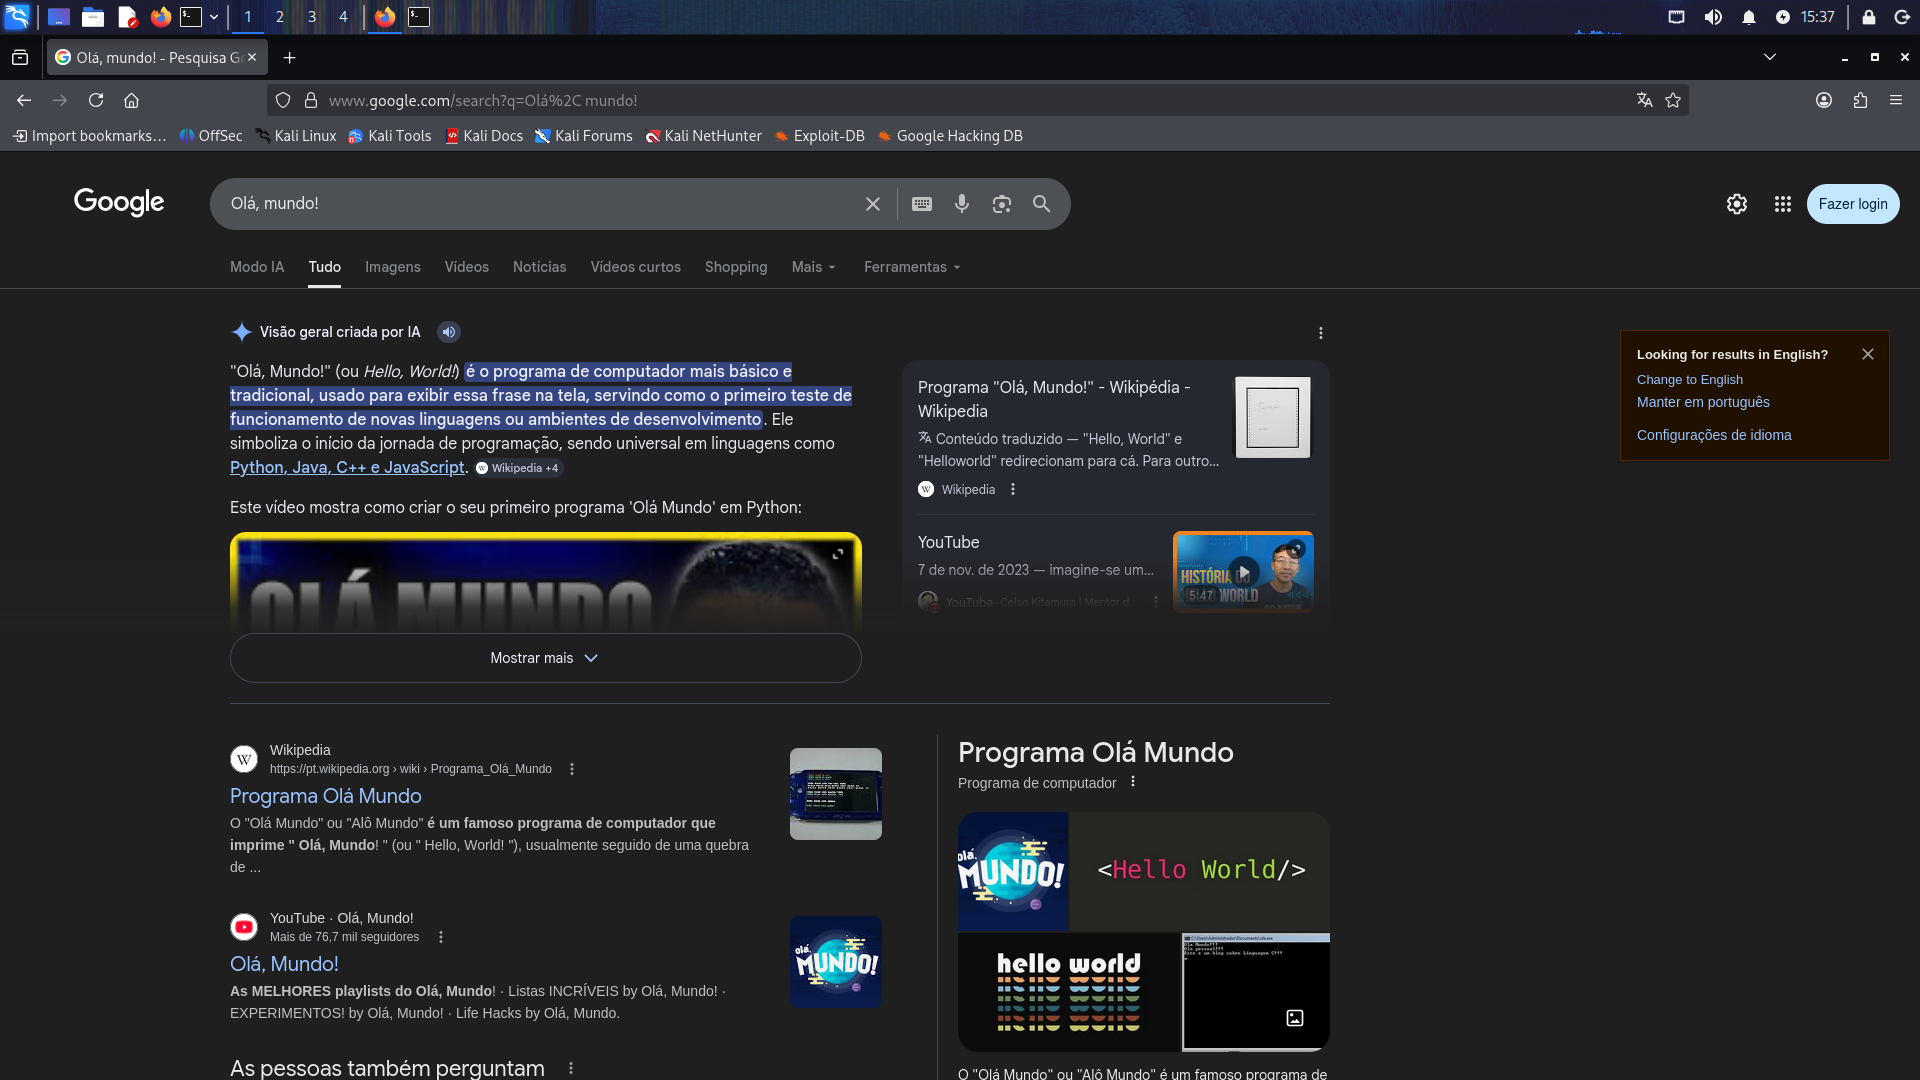
\includegraphics[width=0.99\textwidth]{./fig/fig6.6.png}
  \caption{Execução do comando curl com parâmetros codificados e exibição da resposta HTTP no Terminal}
  \label{fig:fig6.6}
\end{figure}

\newpage

\question[Atividade 6.7]{Encurtando Links e Gerando QR Code no Kali Linux}
\begin{figure}[H]
  \centering
  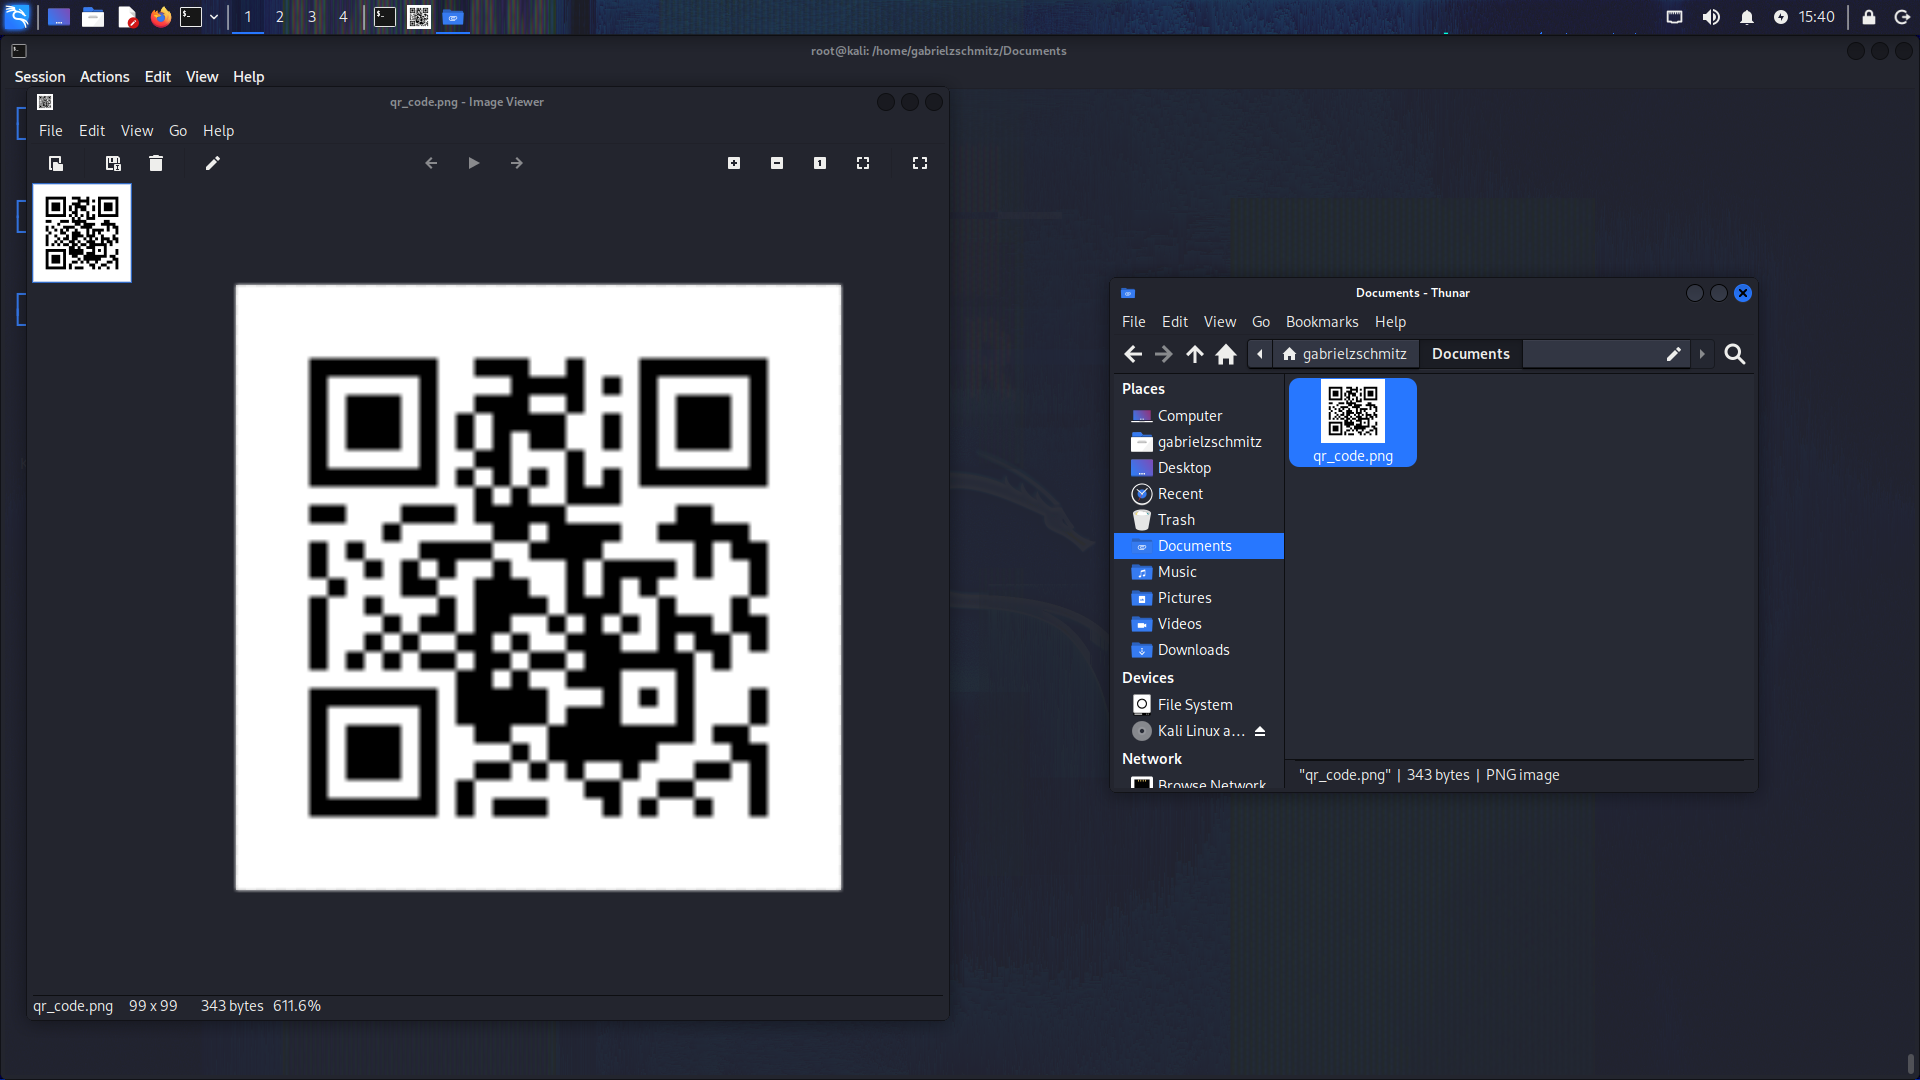
\includegraphics[width=0.99\textwidth]{./fig/fig6.7.png}
  \caption{Criação do QR Code a partir de URL encurtada e visualização do arquivo gerado}
  \label{fig:fig6.7}
\end{figure}

\newpage

\question[Atividade 6.8]{Conhecendo o ataque Clickjacking}
\begin{figure}[H]
  \centering
  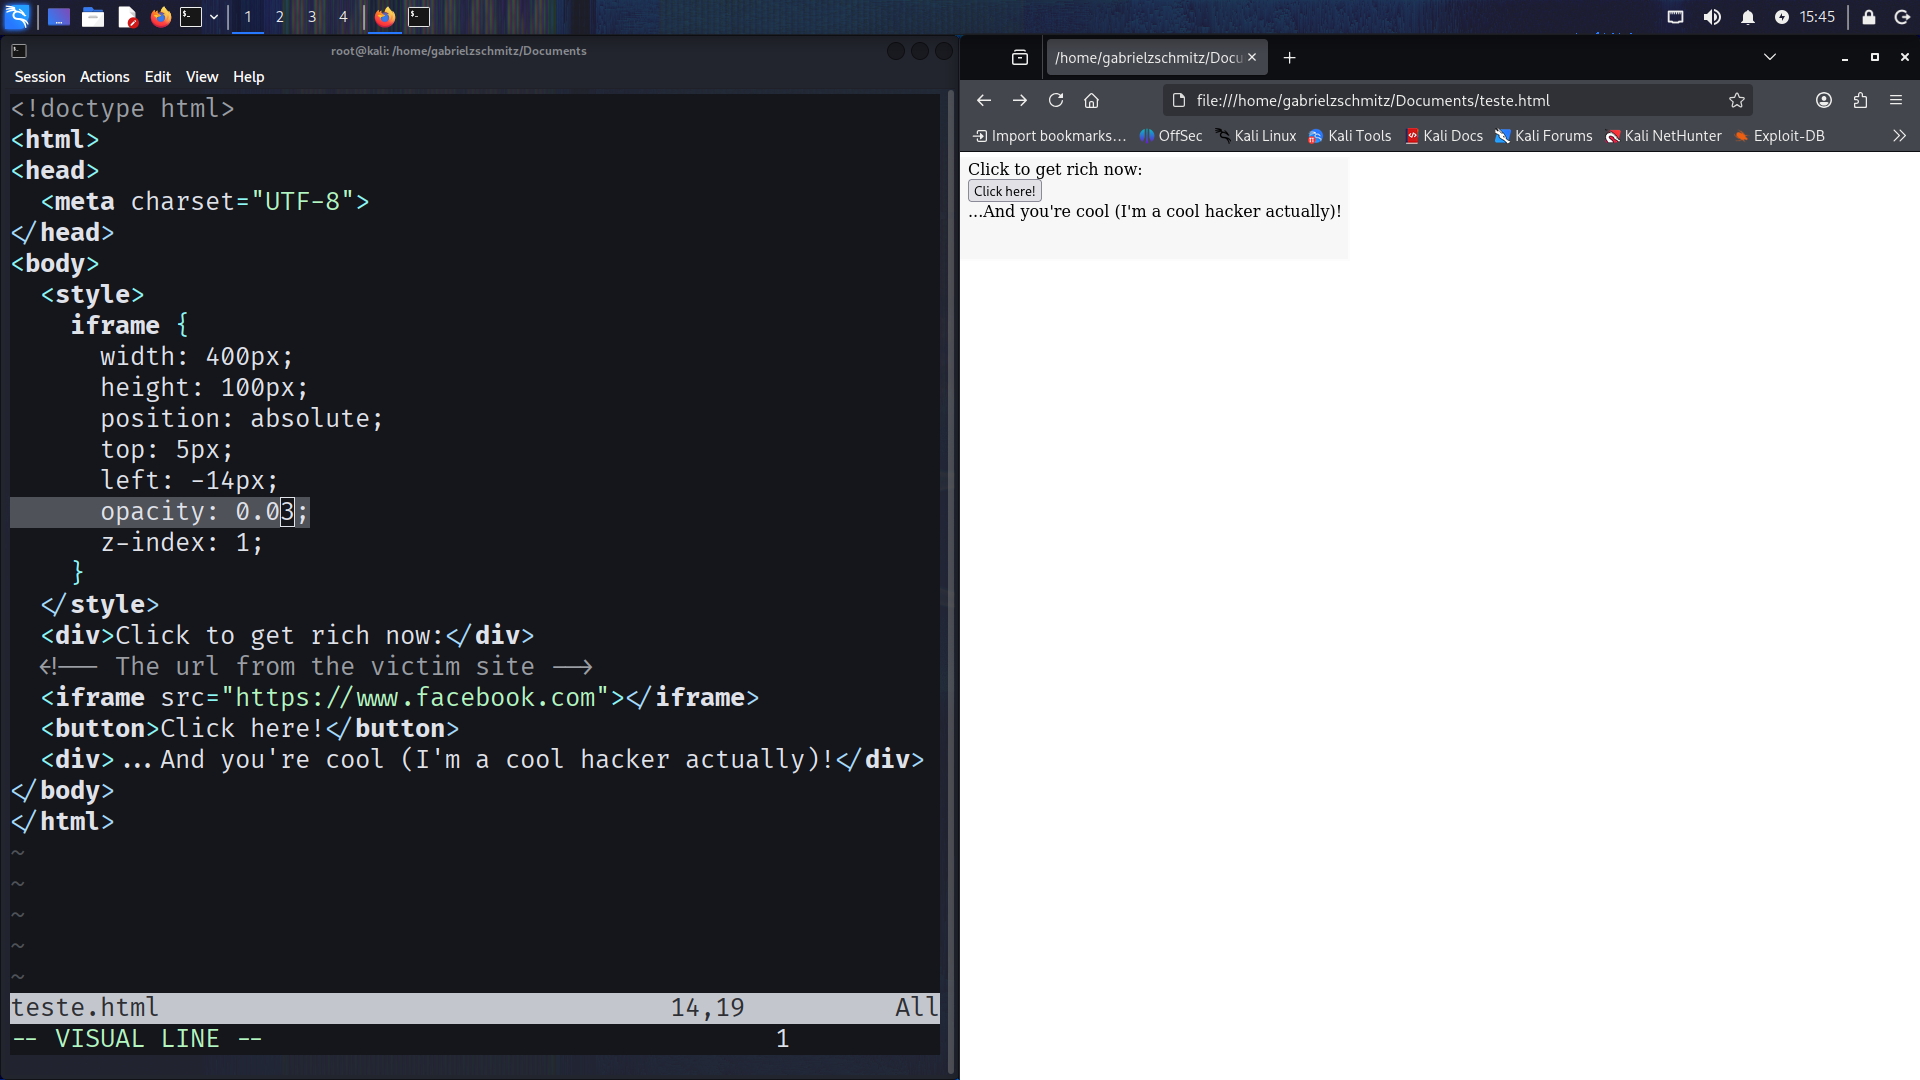
\includegraphics[width=0.99\textwidth]{./fig/fig6.8.png}
  \caption{Demonstração prática do funcionamento do Clickjacking com alteração de opacidade do iframe}
  \label{fig:fig6.8}
\end{figure}

\newpage

\question[Atividade 6.9]{Verificando sites com vulnerabilidade ao Clickjacking}
\begin{figure}[H]
  \centering
  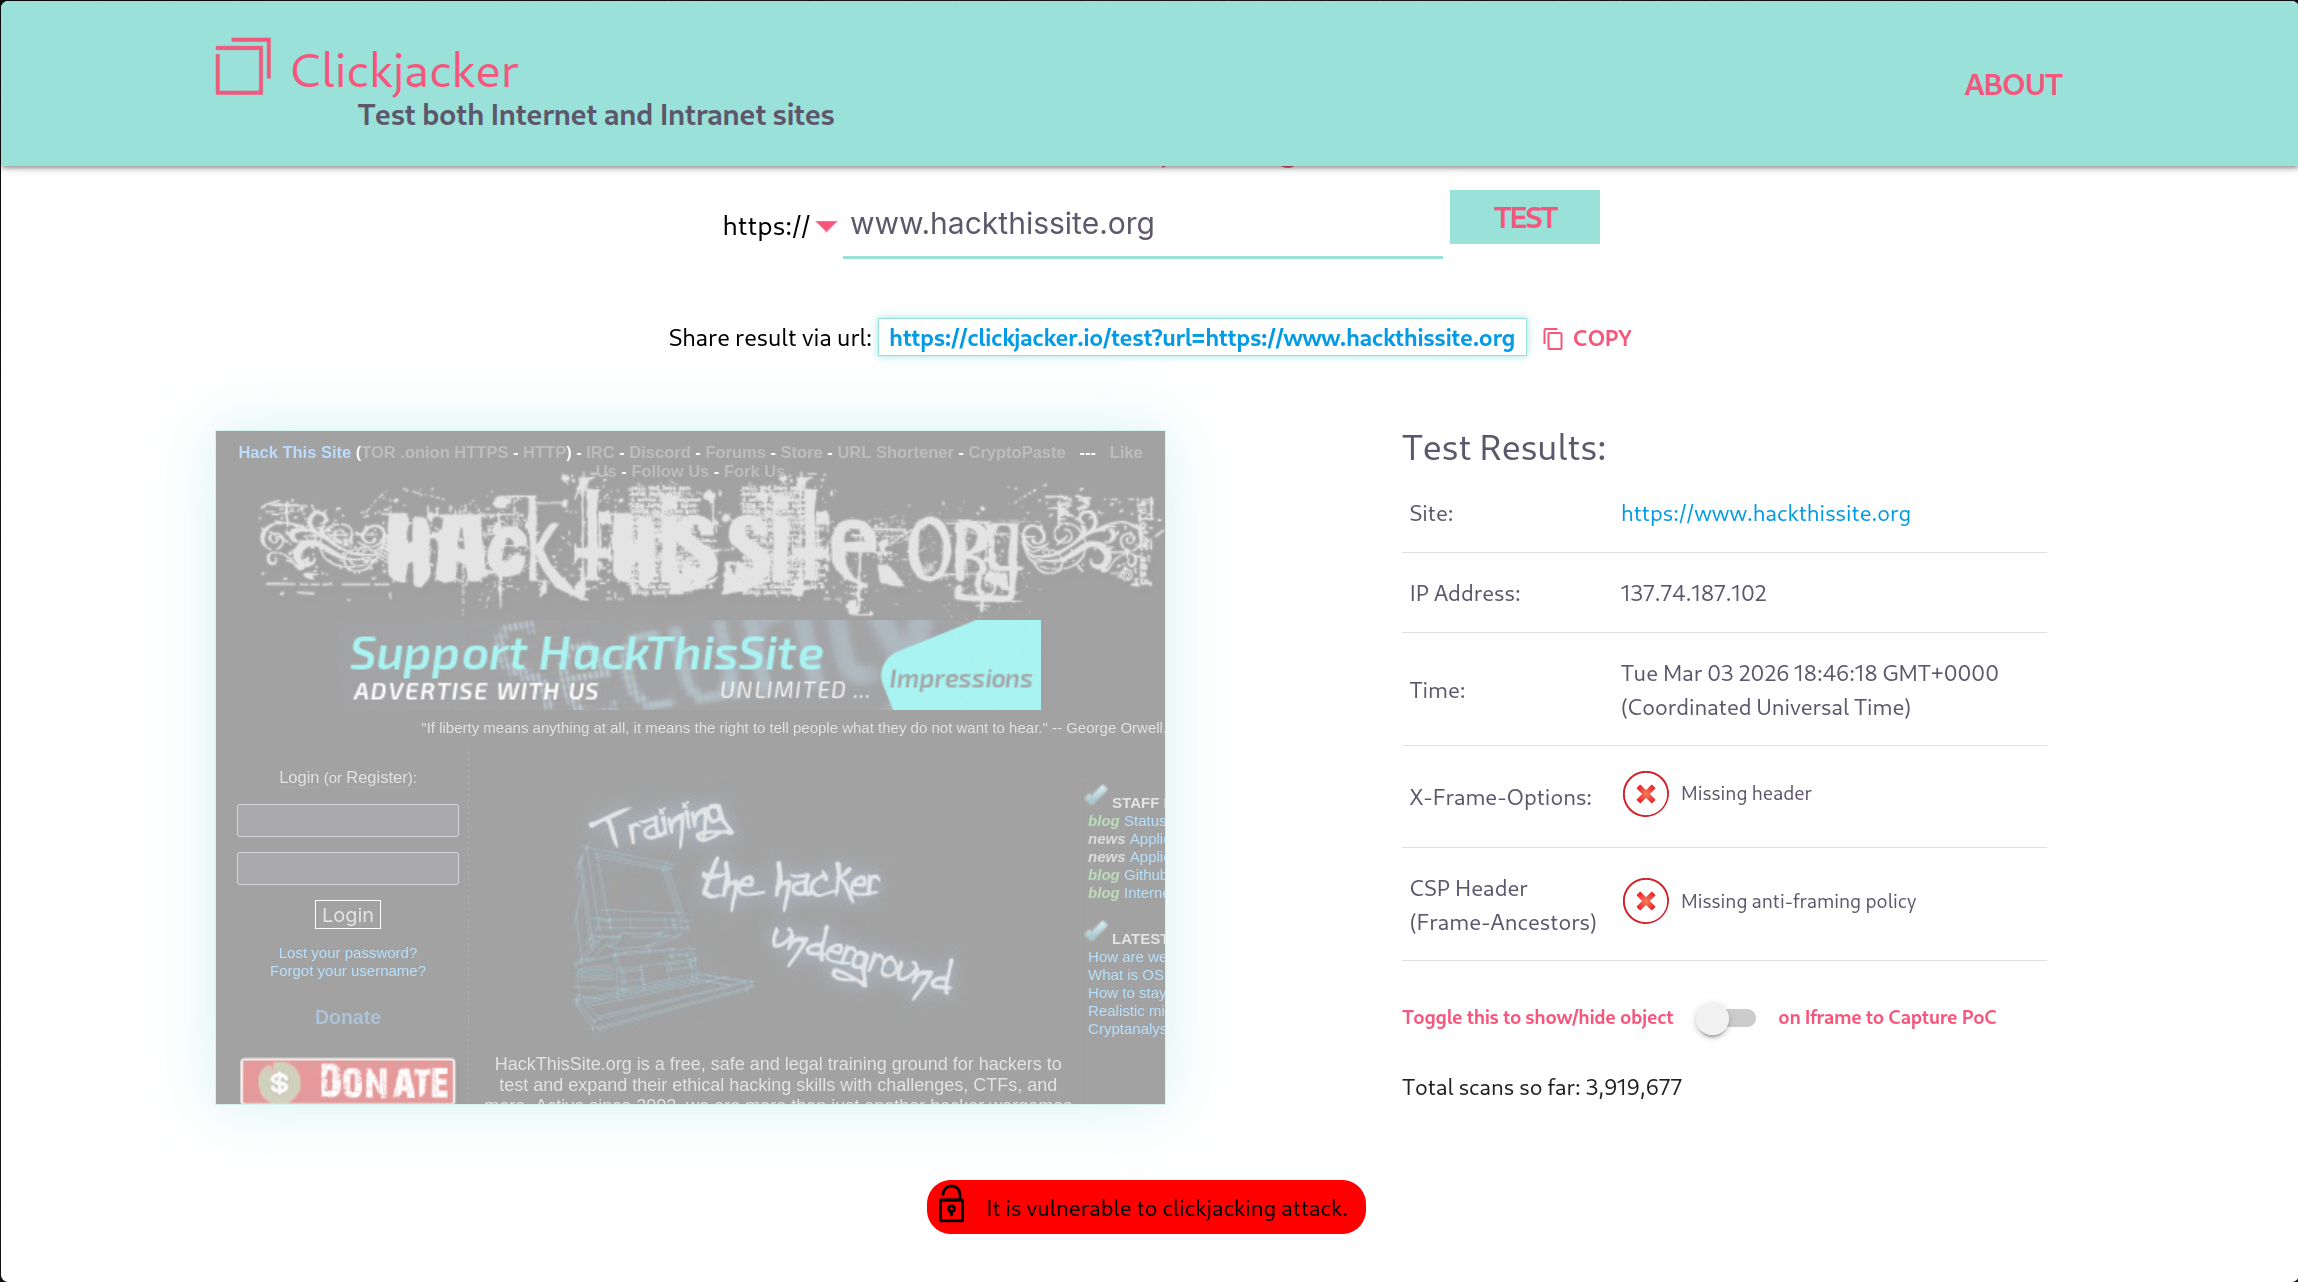
\includegraphics[width=0.99\textwidth]{./fig/fig6.9.png}
  \caption{Resultado da verificação de vulnerabilidade Clickjacking exibindo cabeçalhos X-Frame-Options e CSP}
  \label{fig:fig6.9}
\end{figure}

\newpage

\question[Atividade 6.10]{Explorando o ataque SQL Injection no Kali Linux}
\begin{figure}[H]
  \centering
  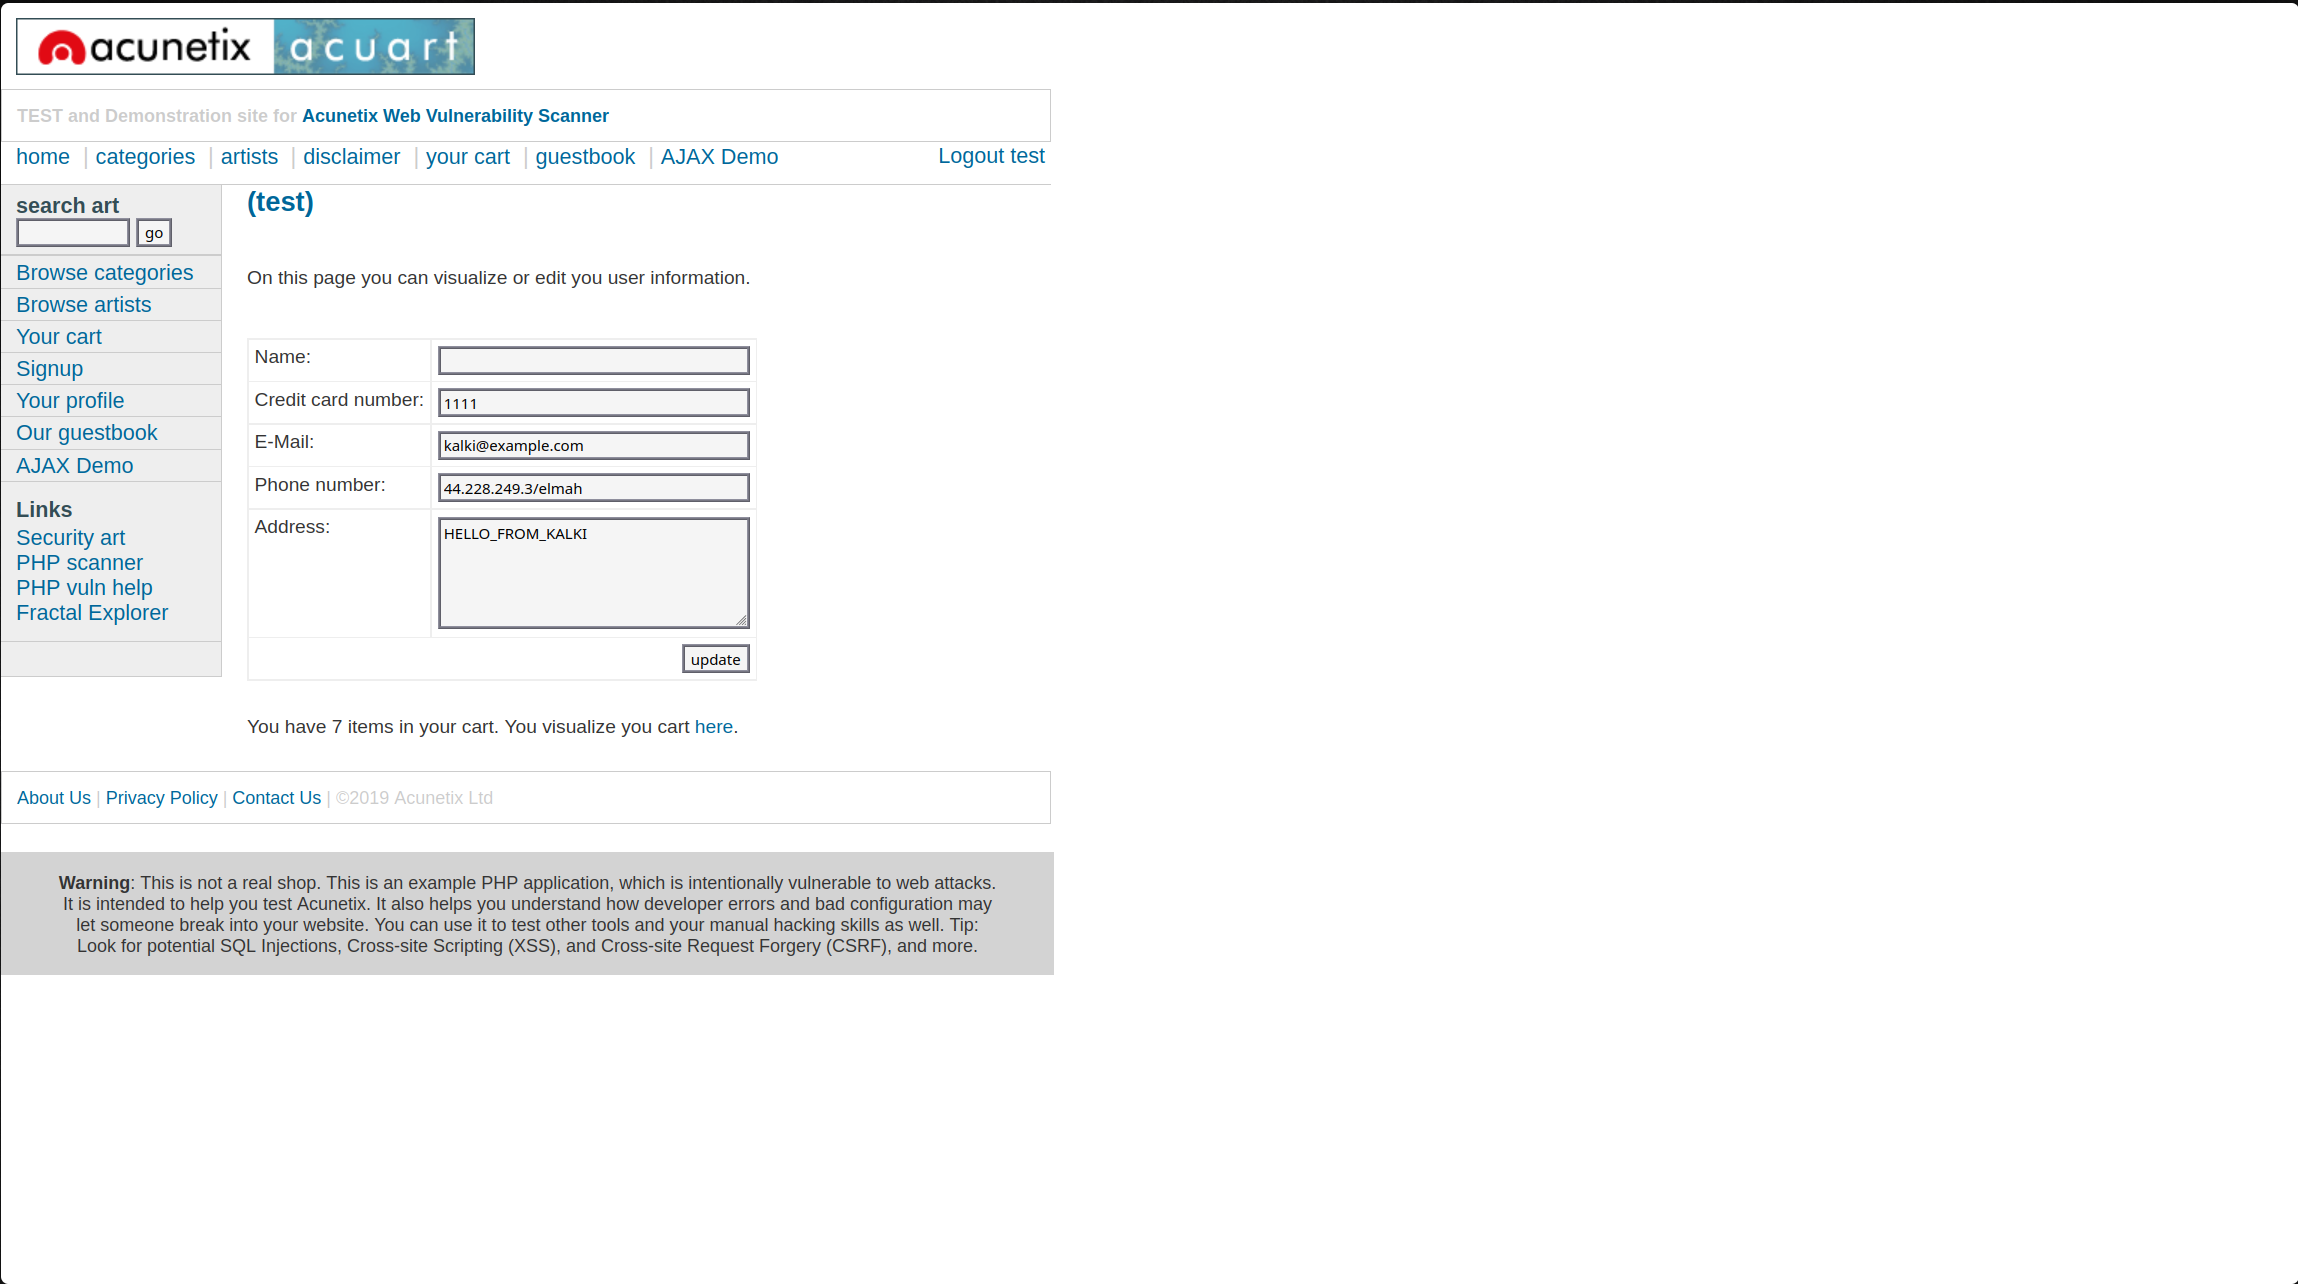
\includegraphics[width=0.99\textwidth]{./fig/fig6.10.png}
  \caption{Identificação de vulnerabilidades SQL Injection e enumeração de bancos de dados com SQLmap}
  \label{fig:fig6.10}
\end{figure}
